\documentclass[border=6pt]{standalone}
\usepackage{tikz}
\usepackage{amsmath}
\begin{document}
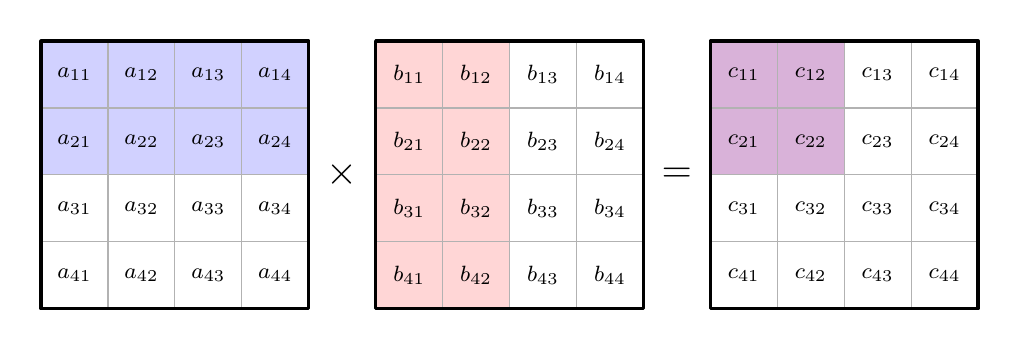
\begin{tikzpicture}[scale=0.85, line join=round]
  \useasboundingbox (-0.2,-0.2) rectangle (14.2,4.2); % identical box

  % --- highlights ---
  \fill[blue!18]   (0,2)  rectangle (4,4);   % A rows 1-2
  \fill[red!16]    (5,0)  rectangle (7,4);   % B cols 1-2
  \fill[violet!30] (10,2) rectangle (12,4);  % C top-left 2x2 block

  \draw[thin,gray!60] (0,0) grid (4,4); \draw[very thick] (0,0) rectangle (4,4);
  \foreach \i in {1,...,4}{\foreach \j in {1,...,4}{
     \node[font=\footnotesize] at (\j-0.5,4-\i+0.5) {$a_{\i\j}$};}}

  \node[font=\Large] at (4.5,2) {$\times$};

  \draw[thin,gray!60] (5,0) grid (9,4); \draw[very thick] (5,0) rectangle (9,4);
  \foreach \i in {1,...,4}{\foreach \j in {1,...,4}{
     \node[font=\footnotesize] at (5+\j-0.5,4-\i+0.5) {$b_{\i\j}$};}}

  \node[font=\Large] at (9.5,2) {$=$};

  \draw[thin,gray!60] (10,0) grid (14,4); \draw[very thick] (10,0) rectangle (14,4);
  \foreach \i in {1,...,4}{\foreach \j in {1,...,4}{
     \node[font=\footnotesize] at (10+\j-0.5,4-\i+0.5) {$c_{\i\j}$};}}
\end{tikzpicture}
\end{document}